\documentclass[10pt]{article}

\def\Type{LessonCaelan}
\def\TypeNum{Lesson 21}
\def\TypeTitle{Continuous Random Variables}
\def\Semester{Fall 2021} %Not Used 
\def\Course{MATH 1190 \& 1210}

\usepackage{preambleDJ}
\usepackage{xcolor} % for blue solutions
\usepackage{pgfplots}

%%%%%%%%%%%% BEGIN DOCUMENT %%%%%%%%%%%%%%%
\begin{document}

\thispagestyle{firstpage}
\pagestyle{otherpages}
\vs{0.4}

\textbf{Intended Learning Outcomes}
After this lesson, you will be able to 

\begin{itemize}
    \item Determine if a random variable is discrete or continuous. (\target{P2})
    \item Define support for a continuous random variable. (\target{P2})
    \item List and apply properties of the probability density function of a continuous random variable. (\target{P2})
    \item Find the formula and the graph of the cumulative distribution function of a continuous random variable. (\target{P2})
\end{itemize}

\vspace{-0.5cm}
\hrulefill

\textbf{\color{blue} Warm Up}\exercise{\bf\color{Orange}P2} Determine whether each of the random variable in the following scenarios is discrete or continuous.

\begin{enumerate}[label=(\alph*)]
    \item The number of arrivals at an emergency room from midnight to 6am on a given day.
    \textcolor{blue}{Discrete, because it counts a finite number of distinct arrivals.}

    \vfill

    \item The temperature of a cup of coffee from a coffee shop.
    \textcolor{blue}{Continuous, because temperature can take any value within a continuous range.}

    \vfill 

    \item The number of boys in a randomly-selected family with 3 children.
    \textcolor{blue}{Discrete, because the number of boys can only be 0, 1, 2, or 3.}

    \vfill
\end{enumerate}

%%%%%%%%%
\newpage%
%%%%%%%%%

{\bf\color{blue}Mini-lecture.} ({\it Smoothing out the Age Historgram})

\begin{center}
    
\includegraphics[scale=0.8]{Spring 2026/Lessons/Week14/images/agehistogram.png}
\end{center}

Suppose $t$ is age in years. We define $p(t)$, the \textbf{probability} density function for age, to be the function that "smoothes out" the age histogram.

If $a$ and $b$ are two ages such that $b\ge a$, then

\[\text{percentage of Population between age $a$ and age $b$}=\int_a^b p(t)\,dt.\]

If the smallest possible age is $0$ and largest possible age is $100$, then 

\[\int_0^{100} p(t)\,dt=1.\]

\fbox{
\begin{minipage}{0.95\textwidth}
\textbf{The Probability Density Function, Properties, and Support}

More generally, for a continuous random variable $X$, its \textbf{probability density function} (PDF) $p(x)$ satisfies that 

\[P(a<X<b)=\int_a^bp(x)\,dx.\]

Analogous to the probability mass function, any probability density function $p(x)$ satisfy the following two important properties.

\begin{enumerate}
    \item For all real numbers $x$, the value of $p(x)$ is always non-negative.
    \item If $a$ is the smallest possible value of $x$ where $p(x)>0$, and $b$ is the largest possible value of $x$ where $p(x)>0$, then 
    \[\int_a^b p(x)\,dx=1.\]
\end{enumerate}

The \textbf{support} of a continuous random variable \(X\) is the smallest interval that contains all number that gives a positive value of the probability density function of \(X\).

\end{minipage}
}

\example{\bf\color{Orange}P2} A person arrives at a bus stop at a random time to catch the next bus. Buses run every 30 minutes without fail, hence the next bus could come any time during the next 30 minutes with evenly distributed probability (a uniform distribution).

Suppose $X$ represents the number of minutes this person waits until the next bus arrives.

\begin{enumerate}[label=(\alph*)]
    \item What is the support of $X$?
    \textcolor{blue}{Support: $[0,30]$ minutes.}

    \vfill

    \item Sketch the graph of the probability density function $p(x)$ of $X$, and find its formula using the properties of the probability density function.
    \textcolor{blue}{
    \[
p(x) = 
\begin{cases} 
\dfrac{1}{30} & \text{for } 0 \leq x \leq 30, \\
0 & \text{otherwise}.
\end{cases}
\]
  } 


\begin{tikzpicture}
\begin{axis}[
    scaled ticks=false,
    ticklabel style={/pgf/number format/fixed}
    axis lines=middle,
    xlabel=$x$, ylabel=$p(x)$,
    ymin=0, ymax=0.05,
    xmin=-5, xmax=35,
    xtick={0,10,20,30},
    ytick={0,0.017,0.0333},
    yticklabels={0,$\frac{1}{60}$,$\frac{1}{30}$},
    width=10cm, height=5cm,
    domain=-5:35,
    samples=2,
    clip=false,
    grid=both, grid style=dashed,
]

% Draw the uniform pdf
\addplot+[thick, domain=0:30] {1/30};

% Draw dashed lines to indicate zero outside
\addplot+[dashed, thick, domain=-5:0] {0};
\addplot+[dashed, thick, domain=30:35] {0};
\end{axis}
\end{tikzpicture}
  \vfill
    
    \item Use $p(x)$ and an integral to find the probability that this person waits for no more than 10 minutes.
    \textcolor{blue}{$P(X \le 10) = \int_0^{10} \frac{1}{30} dx = \frac{10}{30} = \frac{1}{3} \approx 0.333.$}

    \vfill
\end{enumerate}

\exercise{\bf\color{Orange}P2}
Let $X$ be a continuous random variable with probability density function:
\[
p(x) = 
\begin{cases} 
cx & \text{for } 0 \leq x \leq 2, \\
0 & \text{otherwise}.
\end{cases}
\]
\begin{itemize}
\item[(a)] Find the support of $X$.
%
\\
\underline{{\large
\textcolor{blue}{$[0,2]$}
}}
\vfill

\item[(b)] Find the value of the constant $c$.\\
\textcolor{blue}{Solve $\int_0^2 cx \, dx = 1 \implies c \int_0^2 x \, dx = 1 \implies c \cdot \frac{2^2}{2} = 1 \implies c \cdot 2 = 1 \implies c = \frac{1}{2}$.}

\vfill

\item[(c)] Probability $X \le 1.5$:\\
\textcolor{blue}{$P(X \le 1.5) = \int_0^{1.5} \frac{1}{2} x dx = \frac{1}{2} \cdot \frac{(1.5)^2}{2} = \frac{2.25}{4} = 0.5625.$}

\vfill

\item[(d)] Find $b$ such that $P(0\le X\le b)=0.25$:\\
\textcolor{blue}{Solve $\int_0^b \frac{1}{2}x dx = 0.25 \implies \frac{b^2}{4}=0.25 \implies b^2=1 \implies b=1$.}

\vfill
\end{itemize}

%%%%%%%%%
\newpage%
%%%%%%%%%


{\bf\color{blue}Mini-lecture.} Suppose the support of a continuous random variable $X$ is $[a, b]$. The {\bf cumulative distribution function} (CDF) of $X$ is given by
{\color{blue}
\[P(X \leq x) = C(x) = \int_a^x p(t) dt, \quad a\le x\le b.\]
}

In contrast, the PDF and the CDF are also related in the following way. \[p(x)=C'(x)\]

The CDF of a random variable measures how much probability has accumulated up to a given point. It has the following properties.
\begin{enumerate}
    \item $C(x)$ is always non-negative.
    \item $C(x)$ never decreases.
    \item $C(x)=0$ when $x<a$ and $C(x)=1$ when $x>b$.
    \item Assume $c$ and $d$ are within the support of $X$ with $c<d$. The probability of the value of $X$ falls into some interval $(c, d)$ is $C(d)-C(c)$.
\end{enumerate}



\example{\bf\color{Orange}P2} Continuing Example 1, the CDF of $X$ (uniform $[0,30]$):

\textcolor{blue}{For $0\le x\le 30$: $C(x)=\int_0^x \frac{1}{30} dt = \frac{x}{30}$.
\medskip
\[
C(x) = 
\begin{cases} 
0 & \text{for } x < 0, \\
\frac{x}{30} & \text{for } 0 \leq x < 30, \\
1 & \text{for } x \geq 30.
\end{cases}
\]
}
\medskip


\begin{tikzpicture}
\begin{axis}[
    scaled ticks=false,
    ticklabel style={/pgf/number format/fixed}
    axis lines=middle,
    xlabel=$x$, ylabel=$C(x)$,
    ymin=0, ymax=1.3,
    xmin=-5, xmax=45,
    xtick={0,10,20,30,40,45},
    ytick={0,0.5,0.75,1},
    yticklabels={0,0.5,0.75,1},
    width=10cm, height=5cm,
    domain=-5:35,
    samples=2,
    clip=false,
    grid=both, grid style=dashed,
]
% Draw the uniform pdf
\addplot+[thick, domain=0:30] {x/30};
\draw[->, thick, blue] (axis cs:30,1) -- (axis cs:40,1);
% Draw dashed lines to indicate zero outside
% \addplot+[dashed, thick, domain=-5:0] {0};
% \addplot+[dashed, thick, domain=30:35] {0};
\end{axis}
\end{tikzpicture}
\bigskip

\exercise{\bf\color{Orange}P2} The PDF of the continuous random variable $X$ is given below:\\

\

\,\hfill
%
\begin{minipage}[t][0.5in]{0.25\textwidth}
$
p(x) = 
\begin{cases} 
1 & \text{for } 0 \leq x \leq 1, \\
0 & \text{otherwise},
\end{cases}
$
\end{minipage}
%
\hfill
%
\begin{minipage}[t][0.5in]{0.25\textwidth}
\,\\[-0.5in]
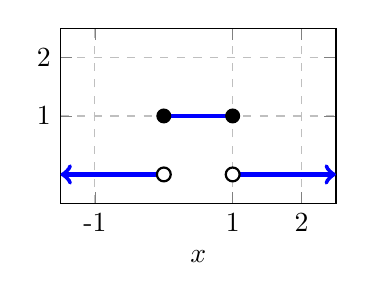
\begin{tikzpicture}
          \begin{axis}[
        %    axis y line = left,
        %    axis x line = bottom,
            xlabel = {$x$},
            xtick       = {-1,1,2},
            xticklabels = {-1,1,2},
            ytick       = {1,2},
            yticklabels = {1,2},
            samples     = 160,
            domain      = -1:3,
            restrict y to domain=-0.1:4,
            xmin = -1.5, xmax = 2.5,
            ymin = -0.5, ymax = 2.5,
            width = 2in, height=1.5in,
            grid=both, grid style=dashed
          ]
          \draw[ultra thick,blue,<-] (-1.5,0) -- (0,0);
          \draw[ultra thick,blue] (0,1) -- (1,1);
          \draw[ultra thick,blue,->] (1,0) -- (2.5,0);
          \filldraw (0,1) circle (2.5pt);
          \filldraw (1,1) circle (2.5pt);
          \filldraw[fill=white, thick] (1,0) circle (2.5pt);
          \filldraw[fill=white, thick] (0,0) circle (2.5pt);
        \end{axis}
\end{tikzpicture}
\end{minipage}
%
\hfill\,\\








\begin{itemize}
\item[(a)]  Use the formula in the mini-lecture to find the CDF $C(x)$ of $X$.


CDF $C(x)$:

\vfill
\textcolor{blue}{
$C(x) = \begin{cases}
0, & x<0\\
x, & 0\le x < 1\\
1, & x \ge 1
\end{cases}$
}

\item[(b)] Sketch the part of the graph of the CDF $C(x)$ within the support of $X$.

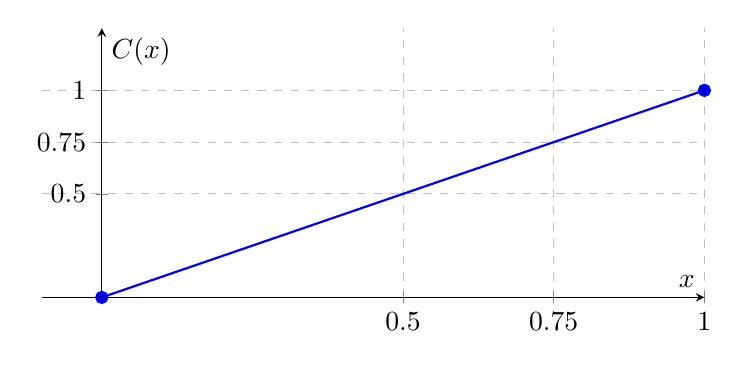
\begin{tikzpicture}
\begin{axis}[
    scaled ticks=false,
%    ticklabel style={/pgf/number format/fixed}
    axis lines=middle,
    xlabel=$x$, ylabel=$C(x)$,
    ymin=0, ymax=1.3,
    xmin=-0.1, xmax=1,
    xtick={0,0.5,0.75,1},
    ytick={0,0.5,0.75,1},
    xticklabels = {0,0.5,0.75,1},
    yticklabels={0,0.5,0.75,1},
    width=10cm, height=5cm,
    domain=-0.5:1,
    samples=2,
    clip=false,
    grid=both, grid style=dashed,
]
% Draw the uniform pdf
\addplot+[thick, domain=0:1] {x};
%\draw[->, thick, blue] (axis cs:1,1) -- (axis cs:2,1);
% Draw dashed lines to indicate zero outside
% \addplot+[dashed, thick, domain=-5:0] {0};
% \addplot+[dashed, thick, domain=30:35] {0};
\end{axis}
\end{tikzpicture}
\bigskip

\begin{minipage}[t]{0.45\textwidth}
    \begin{itemize}
    \item[(c)] Find the number $m$ for which $P(X<m)=0.5$. ({\bf Note:} this number $m$ is called the {\bf median} of $X$.)
    \end{itemize}
\end{minipage}\\

\item[(c)] Median $m$:
\textcolor{blue}{Median $m$ solves $P(X<m)=0.5 \implies m=0.5$.}

\vfill
\end{itemize}
\exercise{\bf\color{Orange}P2} Let $X$ be a continuous random variable. The following graph is either the graph of the PDF $p(x)$ or the CDF $C(x)$.

\begin{center}
     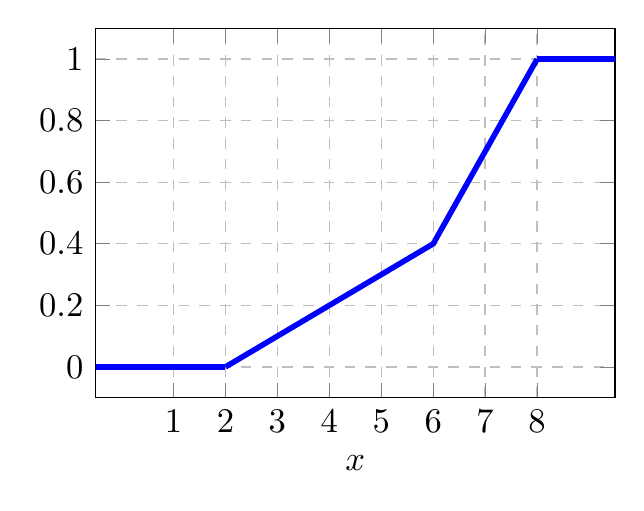
\begin{tikzpicture}[scale=1.25]
           \begin{axis}[
             xlabel={$x$},
             %grid = major,
             xtick       = {1,2,3,4,5,6,7,8},
             xticklabels = {$1$,$2$,$3$,$4$,$5$,$6$,$7$,$8$},
             ytick       = {0, 0.2, 0.4, 0.6, 0.8, 1},
             yticklabels = {$0$, $0.2$, $0.4$, $0.6$, $0.8$, $1$},
             samples     = 320,
             domain      = -1:9.5,
             restrict y to domain=-3.5:2.5,
             xmin = -0.5, xmax = 9.5,
             ymin = -0.1, ymax = 1.1,
             height=2.1in, width=2.7in,
             grid=both, grid style=dashed
           ]
           \draw[ultra thick, blue,-] (2,0) -- (6, 0.4) -- (8,1);
           \draw[ultra thick, blue,-] (-0.5,0) -- (2,0);
           \draw[ultra thick, blue,-] (8, 1) -- (9.5,1);
           %\draw (2,0) circle (1.5pt);
           %\draw (8,0) circle (1.5pt);
           %\draw[blue,fill=blue] (2,0.08) circle (1.5pt);
           %\draw[blue,fill=blue] (8,0.12) circle (1.5pt);
           %\node at (3,0.2) {$p(x)$};
           \end{axis}
     \end{tikzpicture}
     \end{center}

\exercise{\bf\color{Orange}P2} Graph problem: rising curve from $0$ to $1$, asymptotes at 0 and 1.

\begin{enumerate}
    \item[(a)] Determine whether the graph is of $p(x)$ or $C(x)$, and explain why. \\
        \textcolor{blue}{It is a CDF, because it never decreases, starts at 0, ends at 1.}

    \vfill    
    

     \item[(b)] Based on the graph, what is the probability that the value of $X$ falls between 4 and 6?\\
     \textcolor{blue}{$P(4\le X \le 6)=C(6)-C(4)=0.4-0.2=0.2$ (assuming linear scale 0–8).}
         \item[(c)] What is the support of $X$?\\
         \textcolor{blue}{Support: $[2,8]$ (where the CDF increases).}
         \vfill
         
     \item[(d)] Find the formula or the graph of the PDF $p(x)$ or the CDF $C(x)$, which ever is NOT represented by the given graph.\\
\textcolor{blue}{$p(x)=\frac{dC}{dx} = c$ (constant slope)
\begin{align*}
\frac{0.4 - 0}{6-2} &= \frac{0.4}{4} = 0.1 \text{ on the first linear piece and}\\
\frac{1 - 0.4}{8-6} &= \frac{0.6}{2} = 0.3 \text{ on the second linear piece}\\
\end{align*}
\[p(x) = 
\begin{cases}
   0.1  &  \text{ if $2\leq x < 6$}\\
   0.3  & \text{ if $6\leq x < 8$}\\
   0 & \text{ otherwise}
\end{cases}
\]
}
\medskip


\begin{tikzpicture}
\begin{axis}[
    axis lines=middle,
    xlabel=$x$, ylabel=$p(x)$,
    ymin=0, ymax=0.35,
    xmin=0, xmax=10,
    xtick={2,6,8},
    ytick={0,0.1,0.3},
    yticklabels={0,0.1,0.3},
    width=12cm, height=6cm,
    domain=0:10,
    samples=2,
    clip=false,
    grid=both, grid style=dashed
]

% Piecewise function
\addplot+[thick, domain=0:2] {0};
\addplot+[thick, domain=2:6] {0.1};
\addplot+[thick, domain=6:8] {0.3};
\addplot+[thick, domain=8:10] {0};

% Optional: vertical lines to mark jumps
\draw[dashed] (axis cs:2,0) -- (axis cs:2,0.1);
\draw[dashed] (axis cs:6,0) -- (axis cs:6,0.1);
\draw[dashed] (axis cs:6,0.1) -- (axis cs:6,0.3);
\draw[dashed] (axis cs:8,0.3) -- (axis cs:8,0);
\end{axis}
\end{tikzpicture}




     
     \textcolor{blue}{PDF: $p(x)=dC/dx = 0.1$ (constant slope), over $[2,8]$.
     
     
     
     
     
     }
     \vfill
    \end{enumerate}
{\bf\color{blue}Extra Practice 1.} \ltrm{\bf\color{Orange}P2}Consider the following probability density function for a random variable $X$:
\[
    p(x) = 
    \begin{cases} 
    c(1 - x) & \text{for } 0 \leq x \leq 1, \\
    0 & \text{otherwise}.
    \end{cases}
\]

\begin{enumerate}
\item[(a)] Find the value of $c$ making $f$ a valid probability density function.\\
\textcolor{blue}{$\int_0^1 c(1-x) dx = c \left[x-\frac{x^2}{2}\right]_0^1 = c(1-\frac{1}{2})=c \cdot \frac{1}{2}=1 \implies c=2.$}

\item[(b)] Suppose you know $X$ has a $75\%$  chance to fall in the interval $[a,1]$. Find $a$.
\\

\vfill
\textcolor{blue}{Solve $\int_a^1 2(1-x) dx=0.75 \implies \left[2x - x^2\right]_a^1 = 1- (2a  - a^2)=0.75 \implies (2a  -a^2)=0.25$. \\
Solve: 
\begin{align*}
    2a  -a^2&=\frac{1}{4}\\
    8a  -4a^2 &= 1\\
    8a  - 4a^2 - 1 &= 0\\
    4a^2 -8a + 1 &= 0\\
\end{align*}
$a = 1 \pm \frac{\sqrt{3}}{2}$. However, only one of these numbers is in the support.  Hence, $a = 1 - \frac{\sqrt{3}}{2}\approx 0.13$
}

\item[(c)] Suppose you know $X$ has a 25\% chance to fall in the interval $[0,b]$. Find $b$.
\\
25\% chance in $[0,b]$:
\textcolor{blue}{$b = 1 - \frac{\sqrt{3}}{2} \approx 0.13$}
\vfill

\end{enumerate}
{\bf\color{blue}Extra Practice 2.} \ltrm{\bf\color{Orange}P2}
The probability density function of a random variable $X$ is given below:
\[
p(x) = 
\begin{cases} 
3x^2 & \text{for } 0 \leq x \leq 1, \\
0 & \text{otherwise},
\end{cases}
\]
Find and graph the cumulative distribution function $C(x)$.\\
\medskip

\textcolor{blue}{$C(x)=\int_0^x 3t^2 dt = t^3 |_0^x = x^3$.
\[C(x) = \begin{cases}
0, & x<0\\
x^3, & 0\le x < 1\\
1, & x \ge 1
\end{cases}\]
}



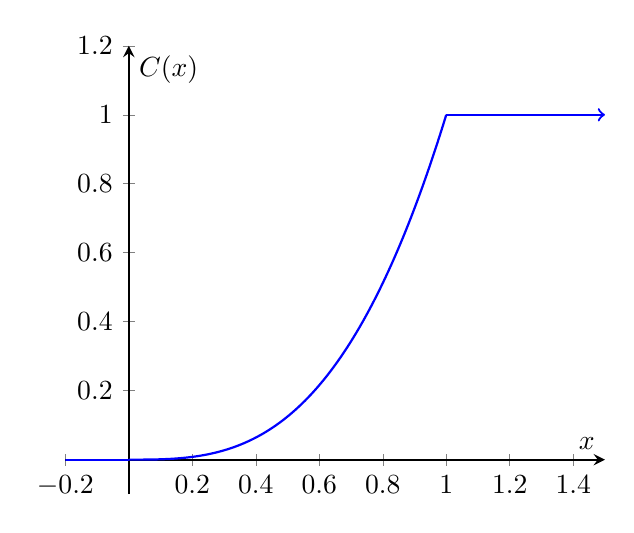
\begin{tikzpicture}
\begin{axis}[
    axis lines=middle,
    xlabel={$x$},
    ylabel={$C(x)$},
    ymin=-0.1, ymax=1.2,
    xmin=-0.2, xmax=1.5,
    domain=0:1,
    samples=100, % increases smoothness
    thick,
]

% x^3 for 0 <= x < 1
\addplot[blue, thick] {x^3};

% Horizontal line for x < 0
\addplot[blue, thick, domain=-0.2:0] {0};

% Horizontal line for x >= 1
\addplot[blue, thick, domain=1:1.5,->] {1};


\end{axis}
\end{tikzpicture}

\end{document}
\end{document}